\documentclass[a4paper,14pt]{extarticle}
\usepackage[english,russian]{babel}
\usepackage{amssymb,amsfonts,amsmath,cite,enumerate,float,indentfirst} 
\usepackage{geometry} % Меняем поля страницы
\geometry{left=2cm}% левое поле
\geometry{right=1.5cm}% правое поле
\geometry{top=1cm}% верхнее поле
\geometry{bottom=2cm}% нижнее поле
\usepackage[utf8]{inputenc}
\usepackage[T2A]{fontenc}
\usepackage{graphicx}
\graphicspath{{pic1/}}
\renewcommand{\theenumi}{\arabic{enumi}}% Меняем везде перечисления на цифра.цифра
 \renewcommand{\labelenumi}{\arabic{enumi}}% Меняем везде перечисления на цифра.цифра
  \renewcommand{\theenumii}{.\arabic{enumii}}% Меняем везде перечисления на цифра.цифра
   \renewcommand{\labelenumii}{\arabic{enumi}.\arabic{enumii}.}% Меняем везде перечисления на цифра.цифра
    \renewcommand{\theenumiii}{.\arabic{enumiii}}% Меняем везде перечисления на цифра.цифра
     \renewcommand{\labelenumiii}{\arabic{enumi}.\arabic{enumii}.\arabic{enumiii}.}% Меняем везде перечисления на цифра.цифра

\usepackage{caption}
\usepackage{color}
\usepackage{xcolor}
\usepackage{listings}

% Цвета для кода

\definecolor{string}{HTML}{B40000} % цвет строк в коде
\definecolor{comment}{HTML}{008000} % цвет комментариев в коде
\definecolor{keyword}{HTML}{1A00FF} % цвет ключевых слов в коде
\definecolor{morecomment}{HTML}{8000FF} % цвет include и других элементов в коде
\definecolor{сaptiontext}{HTML}{FFFFFF} % цвет текста заголовка в коде
\definecolor{сaptionbk}{HTML}{999999} % цвет фона заголовка в коде
\definecolor{bk}{HTML}{FFFFFF} % цвет фона в коде
\definecolor{frame}{HTML}{999999} % цвет рамки в коде
\definecolor{brackets}{HTML}{B40000} % цвет скобок в коде

%%% Отображение кода %%%

% Настройки отображения кода

\lstset{
	language=C++, % Язык кода по умолчанию
	morekeywords={*,...}, % если хотите добавить ключевые слова, то добавляйте
	% Цвета
	keywordstyle=\color{keyword}\ttfamily\bfseries,
	%stringstyle=\color{string}\ttfamily,
	stringstyle=\ttfamily\color{red!50!brown},
	commentstyle=\color{comment}\ttfamily\itshape,
	morecomment=[l][\color{morecomment}]{\#}, 
	% Настройки отображения     
	breaklines=true, % Перенос длинных строк
	basicstyle=\ttfamily\footnotesize, % Шрифт для отображения кода
	backgroundcolor=\color{bk}, % Цвет фона кода
	frame=lrb,xleftmargin=\fboxsep,xrightmargin=-\fboxsep, % Рамка, подогнанная к заголовку
	rulecolor=\color{frame}, % Цвет рамки
	tabsize=3, % Размер табуляции в пробелах
	% Настройка отображения номеров строк. Если не нужно, то удалите весь блок
	%numbers=left, % Слева отображаются номера строк
	%stepnumber=1, % Каждую строку нумеровать
	%numbersep=5pt, % Отступ от кода 
	%numberstyle=\small\color{black}, % Стиль написания номеров строк
	% Для отображения русского языка
	extendedchars=true,
	literate={Ö}{{\"O}}1
	{Ä}{{\"A}}1
	{Ü}{{\"U}}1
	{ß}{{\ss}}1
	{ü}{{\"u}}1
	{ä}{{\"a}}1
	{ö}{{\"o}}1
	{~}{{\textasciitilde}}1
	{а}{{\selectfont\char224}}1
	{б}{{\selectfont\char225}}1
	{в}{{\selectfont\char226}}1
	{г}{{\selectfont\char227}}1
	{д}{{\selectfont\char228}}1
	{е}{{\selectfont\char229}}1
	{ё}{{\"e}}1
	{ж}{{\selectfont\char230}}1
	{з}{{\selectfont\char231}}1
	{и}{{\selectfont\char232}}1
	{й}{{\selectfont\char233}}1
	{к}{{\selectfont\char234}}1
	{л}{{\selectfont\char235}}1
	{м}{{\selectfont\char236}}1
	{н}{{\selectfont\char237}}1
	{о}{{\selectfont\char238}}1
	{п}{{\selectfont\char239}}1
	{р}{{\selectfont\char240}}1
	{с}{{\selectfont\char241}}1
	{т}{{\selectfont\char242}}1
	{у}{{\selectfont\char243}}1
	{ф}{{\selectfont\char244}}1
	{х}{{\selectfont\char245}}1
	{ц}{{\selectfont\char246}}1
	{ч}{{\selectfont\char247}}1
	{ш}{{\selectfont\char248}}1
	{щ}{{\selectfont\char249}}1
	{ъ}{{\selectfont\char250}}1
	{ы}{{\selectfont\char251}}1
	{ь}{{\selectfont\char252}}1
	{э}{{\selectfont\char253}}1
	{ю}{{\selectfont\char254}}1
	{я}{{\selectfont\char255}}1
	{А}{{\selectfont\char192}}1
	{Б}{{\selectfont\char193}}1
	{В}{{\selectfont\char194}}1
	{Г}{{\selectfont\char195}}1
	{Д}{{\selectfont\char196}}1
	{Е}{{\selectfont\char197}}1
	{Ё}{{\"E}}1
	{Ж}{{\selectfont\char198}}1
	{З}{{\selectfont\char199}}1
	{И}{{\selectfont\char200}}1
	{Й}{{\selectfont\char201}}1
	{К}{{\selectfont\char202}}1
	{Л}{{\selectfont\char203}}1
	{М}{{\selectfont\char204}}1
	{Н}{{\selectfont\char205}}1
	{О}{{\selectfont\char206}}1
	{П}{{\selectfont\char207}}1
	{Р}{{\selectfont\char208}}1
	{С}{{\selectfont\char209}}1
	{Т}{{\selectfont\char210}}1
	{У}{{\selectfont\char211}}1
	{Ф}{{\selectfont\char212}}1
	{Х}{{\selectfont\char213}}1
	{Ц}{{\selectfont\char214}}1
	{Ч}{{\selectfont\char215}}1
	{Ш}{{\selectfont\char216}}1
	{Щ}{{\selectfont\char217}}1
	{Ъ}{{\selectfont\char218}}1
	{Ы}{{\selectfont\char219}}1
	{Ь}{{\selectfont\char220}}1
	{Э}{{\selectfont\char221}}1
	{Ю}{{\selectfont\char222}}1
	{Я}{{\selectfont\char223}}1
	{і}{{\selectfont\char105}}1
	{ї}{{\selectfont\char168}}1
	{є}{{\selectfont\char185}}1
	{ґ}{{\selectfont\char160}}1
	{І}{{\selectfont\char73}}1
	{Ї}{{\selectfont\char136}}1
	{Є}{{\selectfont\char153}}1
	{Ґ}{{\selectfont\char128}}1
	{\{}{{{\color{brackets}\{}}}1 % Цвет скобок {
	{\}}{{{\color{brackets}\}}}}1 % Цвет скобок }
}
% Для настройки заголовка кода

\DeclareCaptionFont{white}{\color{сaptiontext}}
\DeclareCaptionFormat{listing}{\parbox{\linewidth}{\colorbox{сaptionbk}{\parbox{\linewidth}{#1#2#3}}\vskip-4pt}}
\captionsetup[lstlisting]{format=listing,labelfont=white,textfont=white}
\renewcommand{\lstlistingname}{Код} % Переименование Listings в нужное именование структуры
% Для отображения кода формата xml

\lstdefinelanguage{XML}
{
	morestring=[s]{"}{"},
	morecomment=[s]{?}{?},
	morecomment=[s]{!--}{--},
	commentstyle=\color{comment},
	moredelim=[s][\color{black}]{>}{<},
	moredelim=[s][\color{red}]{\ }{=},
	stringstyle=\color{string},
	identifierstyle=\color{keyword}
}

\newcommand{\imgh}[3]
{
	\begin{figure}[h]
		\center{\includegraphics[width=#1]{#2}}
		\caption{#3}
		\label{ris:#2}
	\end{figure}
}

\begin{document}
	\begin{titlepage}
	\newpage
	
	\begin{center}
		Университет ИТМО \\
	\end{center}
	
	\vspace{1em}
	
	\begin{center}
		\Large Кафедра Мехатроники \\ 
	\end{center}
	
	\vspace{8em}
	
	\begin{center}
		\textsc{\textbf{Курсовой проект:\linebreak \newline \huge "НАЗВАНИЕ КУРСОВОГО ПРОЕКТА}}
	\end{center}
	
	\vspace{14em}
\begin{flushright}
	\begin{tabular}{rl}
		Преподаватель: & Д.В. Куприянов \\
		Выполнили: & Иван Иванов  \\
		&  Пётр Петров \\
		&  Сидор Сидоров \\
		Группа: & P4444\\
	\end{tabular}
\end{flushright}
	

	
	
	\vspace{\fill}
	
	\begin{center}
		Санкт-Петербург \\2017
	\end{center}
	
\end{titlepage}% это титульный лист
	\newpage
	\tableofcontents 
	
	\newpage
	
	\begin{center}	
		\section{Введение}
		
		\end{center}
\subsection{Описание проекта}
Что же сделано?
\subsection{Актуальность}
Зачем оно нужно?
\subsection{Цель работы}
Каким образом и что нового было изучено?
		\newpage
		\begin{center}	
		\section{Подготовка к работе}
			\end{center}
		\subsection{Проведение опроса об актуальности }
	Если нужно
		
		\subsection{Принципы работы составных элементов системы}
	Если нужно
	
	\begin{figure}[H] 
		\center 
		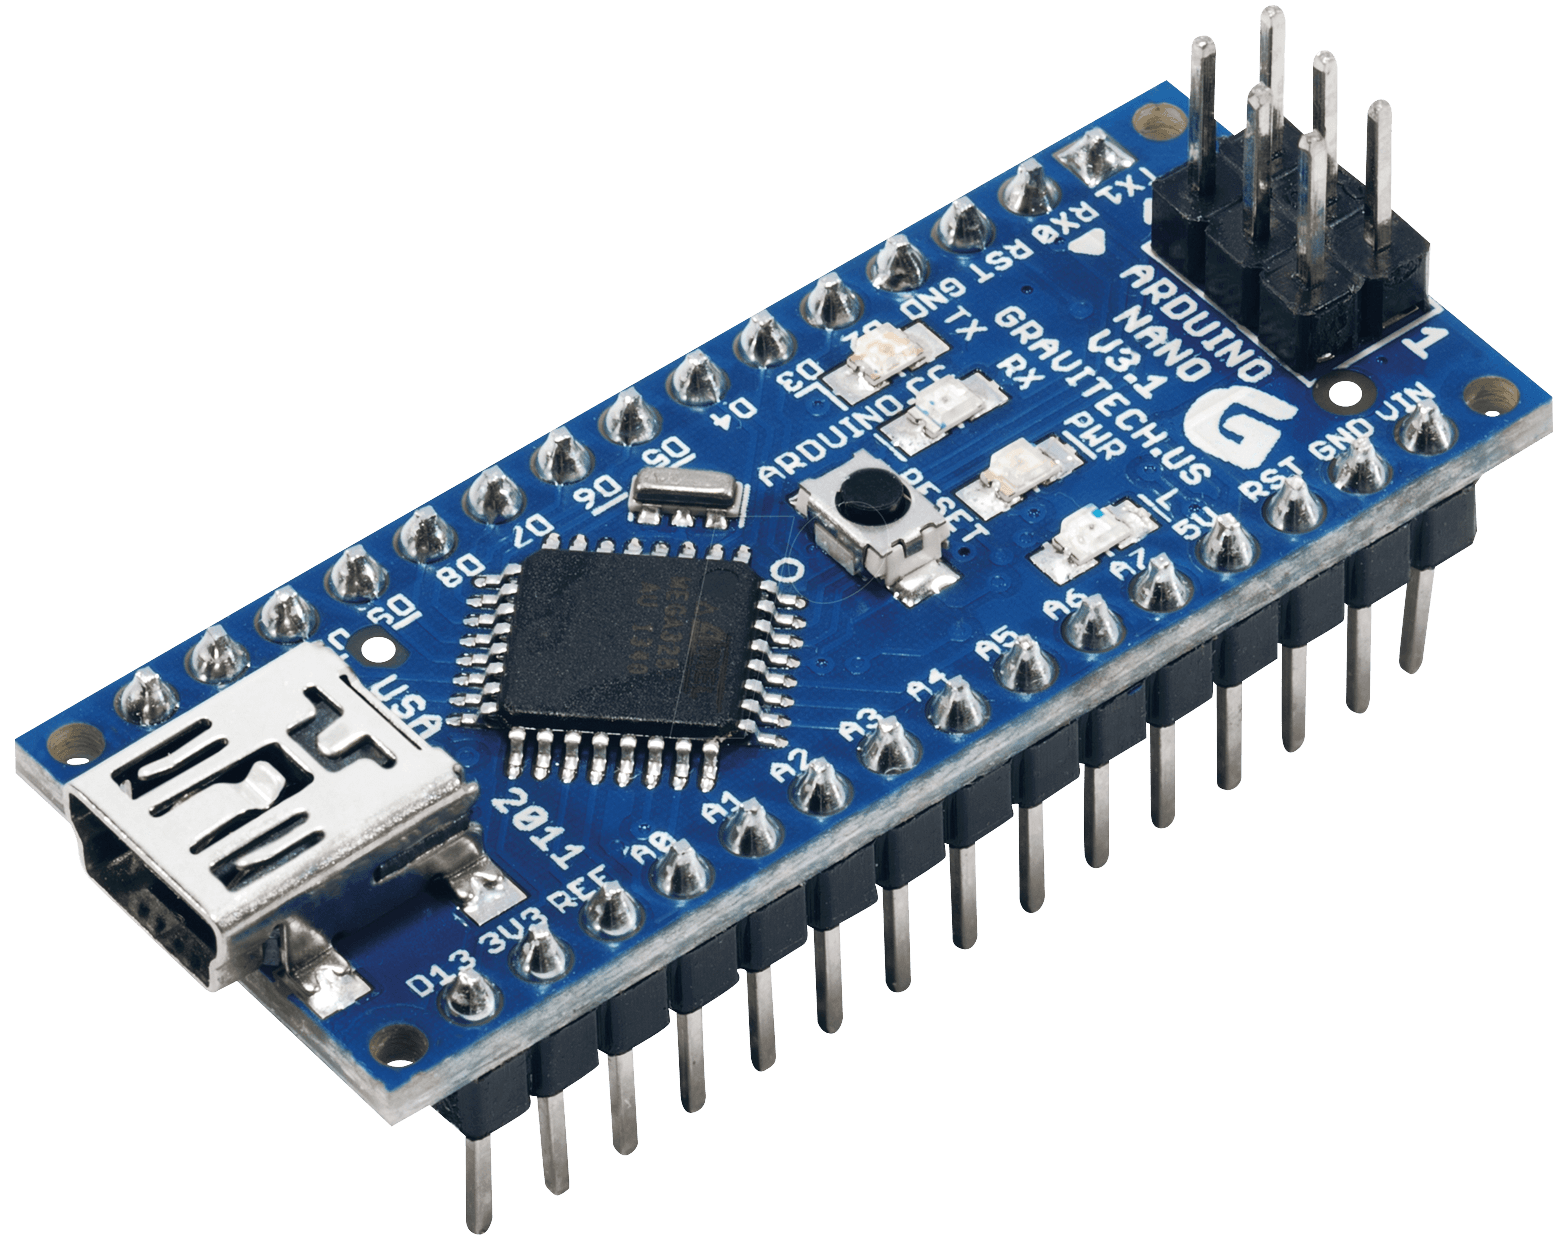
\includegraphics[width=0.7\linewidth]{principle.png} %тут в конце адрес картинки
		\caption{Текст под картинкой} 
		\label{image:principle}   %% внутренняя ссылка на картинку в рамках документа
	\end{figure}
	 В работы был использован элемент (рис.\ref{image:principle}),.
	

	
	\newpage
		\begin{center}	
				\section{Выбор комплектующих. Разработка корпуса}
		\end{center}
		\subsection{Выбор комплектующих}
	Текст 
		\newline

	
		\subsection{Разработка корпуса}
		

   
		 
		
	\newpage
		\begin{center}	
				\section{Схема подключения компонентов}
		\end{center}
	\subsection{Подключение}

\subsection{Особенность чего-то}

	\newpage
		\begin{center}	
				\section{Программный код мультиключа}
		\end{center}
    	\subsection{Описание алгоритма}
    Описание.
    	\newline
    	\newline
    	Полный код прикреплён в приложении \ref{some-code}.
    	
    
	
	
	\newpage
\begin{center}
	\section{Заключение}
	\end{center}

\subsection{Конечный результат. Итоги работы}

 Текст
	\newline
	\newline
Текст
	\newline
	\newline
Текст
	\newline
	\newline
Вывод
	\newpage

\addcontentsline{toc}{section}{Список используемой литературы}

%далее сам список используевой литературы
\begin{thebibliography}{}
	\bibitem{litlink1}  geektimes.ru/post/258674/  -  "Домофонный мультиключ и всё про имитацию «таблеток»"
	\bibitem{litlink2}  robocraft.ru/blog/arduino/82.html  -  "Программирование Arduino - EEPROM"
	\bibitem{litlink3}  electromost.com  -  "Протокол для электронных ключей RW1990"
	\bibitem{litlink4}  soltau.ru  -  "Инструкция по чтению и записи ключа iButton (1-wire) с помощью Arduino"
	\bibitem{litlink5}  easyelectronics.ru -  "Работа в Eagle Cad"
\end{thebibliography}



	\newpage

\addcontentsline{toc}{section}{Приложение}

\begin{center}
    \huge    Приложение
\end{center}

\begin{minted}{python}
def function(arg1, arg2="stroka", *, arg3=5, **kwargs):
    return arg1 + arg2 + arg3 + kwargs["arg4"]
\end{minted}

	
	
\end{document}
